\documentclass[a4paper,12pt]{article}

% Import the deliverable package from common directory
\usepackage{../common/deliverable}

% Tell LaTeX where to find graphics files
\graphicspath{{../common/logos/}{./figures/}{../}}

\usepackage{xspace}
\usepackage{lipsum}
\usepackage{listings}
\lstset{
    language=C++,
    basicstyle=\ttfamily\footnotesize,
    keywordstyle=\color{blue},
    commentstyle=\color{gray},
    stringstyle=\color{red},
    breaklines=true,
    frame=single,
    numbers=left,
    numberstyle=\tiny,
    showstringspaces=false
}

% Set the deliverable number (without the D prefix, it's added automatically)
\setdeliverableNumber{1.1}

% Begin document
\begin{document}

% Create the title page with the title as argument
\maketitlepage{External libraries integration}

\newpage

% Main Table using the new environment and command
\begin{deliverableTable}
    \tableEntry{Deliverable title}{External libraries integration}
    \tableEntry{Deliverable number}{D1.1}
    \tableEntry{Deliverable version}{0.1}
    \tableEntry{Date of delivery}{31/07/2025}
    \tableEntry{Actual date of delivery}{\today}
    \tableEntry{Nature of deliverable}{Other}
    \tableEntry{Dissemination level}{Public}
    \tableEntry{Work Package}{WP1}
    \tableEntry{Partner responsible}{INPT}
\end{deliverableTable}

% Abstract and Keywords Section
\begin{deliverableTable}
    \tableEntry{Abstract}{This document describes the integration of
        external libraries in the deal.II finite element library, namely
        the MUMPS sparse direct solver, the PSCToolkit iterative solver
        and the GMSH three-dimensional finite element mesh generator.}
    \tableEntry{Keywords}{API; solvers; mesh; parallelism; interfaces}
\end{deliverableTable}

\newpage

\begin{documentControl}
    \addVersion{0.1}{15/07/2025}{Alfredo Buttari}{Initial draft}
    \addVersion{0.2}{22/07/2025}{Marco Feder}{Preliminary experimental results}
    \addVersion{0.3}{23/07/2025}{Fabio Durastante}{Integration of PSCToolkit}
    \addVersion{0.4}{28/07/2025}{Marco Feder}{Integration of distributed GMSH capabilities}
    \addVersion{0.5}{29/07/2025}{Alfredo Buttari}{Review and reference
    added}
    \addVersion{1.0}{[Date]}{[Author name]}{Final version}
\end{documentControl}

\subsection*{{Approval Details}}
Approved by: [Name] \\
Approval Date: [Date]

\subsection*{{Distribution List}}
\begin{itemize}
    \item [] - Project Coordinators (PCs)
    \item [] - Work Package Leaders (WPLs)
    \item [] - Steering Committee (SC)
    \item [] - European Commission (EC)
\end{itemize}

\vspace*{2cm}

\disclaimer

\newpage

\tableofcontents % Automatically generated and hyperlinked Table of Contents

\newpage

\section{{Introduction}}

The objective of the dealii-X Work Package 1 is to enhance the
capabilities of the deal.ii finite element library through the use of
some external libraries, namely, the MUMPS and PSCToolkit solvers and
the GMSH three-dimensional finite element mesh generator. MUMPS is a
parallel direct solver for sparse linear systems, i.e., it achieves
the solution by computing the factorization (LU, $LDL^T$ or Cholesky,
depending of the problem type) of the system matrix and using the
resulting factors in forward/backward substitution operations. One of
the objectives of WP1 is to assess the effectiveness of some of the
recent advanced features of MUMPS such as the block low-rank
approximations or the mixed-precision computations on problems issued
from the simulation of human body organs. PSCToolkit implements
multiple parallel iterative solvers of the Krylov family for the
solution of large scale sparse linear systems. These methods are, by
nature, scalable; furthermore, PSCToolkit provides efficient algebraic
multigrid preconditioners to improve the convergence. Finally, WP1
deals with the integration of the GMSH three-dimensional finite
element meshing package in order to optimize the mesh generation at
large scale.

\subsection{{Purpose of the Document}}
This document describes the integration of the above-mentioned
external packages, the corresponding API within the deal.ii framework
and the features that are exposed to enable experimenting with
advanced features in the context of the dealii-X project.

% \subsection{Objectives of Work Package 1 (WP1)}

% The main objective of Work Package 1 (WP1) is to serve as the foundation
% for the dealii-X Centre of Excellence by enhancing and expanding the
% capabilities of the deal.II library to address the challenges of exascale
% computing and facilitate the creation of advanced digital twins of human
% organs.

% The key steps of WP1 include:
% \begin{itemize}
% \item Extending and improving the exascale capabilities of deal.II;
% \item Improving pre-exascale modules of the deal.II library;
% \item Developing an experimental polygonal discretization module for
%   deal.II;
% \item Integrating PSCToolkit within deal.II;
% \item Integrating MUMPS within deal.II.
% \end{itemize}

% Specifically, the sub-work packages aim to:
% \begin{itemize}
% \item \textbf{WP1.1 (Lead RUB)}: Develop matrix-free computational
%   methods optimized for GPU architectures and enhance the scalability
%   of solvers;
%     \item \textbf{WP1.2 (Lead UNIPI)}: Improve the gmsh API, develop a
%       generalized interface for coupling operators, enhance reduced
%       order modelling capabilities, integrate low-rank approximation
%       methods, and develop block preconditioners;
%     \item \textbf{WP1.3 (Lead SISSA)}: Introduce and parallelize
%       polygonal discretization methods within deal.II and develop
%       related multigrid techniques;
%     \item \textbf{WP1.4 (Lead UNITOV)}: integrate PSCToolkit into
%       deal.II, leveraging GPU computing and developing efficient
%       preconditioners for multiphysics problems;
%     \item \textbf{WP1.5 (Lead INPT)}: Integrate the MUMPS solver
%       directly into deal.II for use in multigrid methods and explore
%       low-rank and mixed-precision techniques;
% \end{itemize}

% In summary, WP1 is dedicated to developing and integrating fundamental
% software components within the deal.II library and external libraries,
% with a strong emphasis on enabling exascale computation for the
% digital twin applications in WP2.

% \subsection{Purpose and Scope of this Report (Deliverable D1.1)}

% The purpose of this report is to make a comprehensive analysis of the
% development that are necessary to integrate external libraries,
% namely, MUMPS, PSCToolkit and GMSH, within the deal.II package. 


% \subsection{{Structure of the Document}}
% \begin{itemize}
% \item Section \ref{sec:section2}: [Section Title]
% \item Section \ref{sec:section3}: [Section Title]
% \item Section \ref{sec:section4}: [Section Title]
% \item Section \ref{sec:section5}: [Section Title]
% \item Section \ref{sec:section6}: [Section Title]
% \end{itemize}

\newpage

\section{MUMPS}
\label{sec:section2}

\subsection{Existing interface}

The deal.II package used to support a direct MUMPS integration in the
past. This support was subsequently remove in favor of an indirect use
of MUMPS through the PETSc library. As a first step towards the
objectives of WP1 of the dealii-X project, this support was reverted,
as documented in Pull Request \#18255
(\url{https://github.com/dealii/dealii/pull/18255}) which has been
subsequently merged in the main branch. This minimalistic interface
includes a number of basic tests.


\subsection{Implemented improvements in the MUMPS support}

The basic deal.II MUMPS interface did not include support for
distributed-memory parallelism, which means that the system matrix and
right-hand side(s) were entirely assembled on the master process where
the subsequent phases (symbolic analysis, factorization and
backward/forward substitution) take place; not only this might be
infeasible due to memory limitations but it severely limits the
performance of the sparse direct solver. The MUMPS integration in
deal.ii was extended to support distributed memory parallelism through
the use of distributed matrix and vector datatypes as defined in the
deal.ii PETSc and Trilinos wrappers. This allows for a completely
parallel initialization of the MUMPS data structure (that includes the
system matrix and the right-hand sides) prior to the symbolic
analysis, numerical factorization and forward/backward substitution.

Setting-up MUMPS internal configuration parameters was not possible in
original deal.II MUMPS interface which, therefore, had to be
extended to enable the use of the more advanced features of the MUMPS
solver; these include the Block Low-Rank approximations, the GPU
support and numerous other parameters that allow for fine-tuning both
the performance and the numerical robustness of the solver. This
extension was achieved by adding a \texttt{AdditionalData} object
to the constructor of the MUMPS solver class that takes the desired
values for selected solver parameters.

The work related to above-mentioned extension is documented in pull
request \#18497 (\url{https://github.com/dealii/dealii/pull/18497})
which was eventually merged in the master deal.ii branch.

Furthermore, the deal.ii documentation was updated with a detailed description
of the MUMPS API within deal.ii:

\url{https://dealii.org/developer/doxygen/deal.II/classSparseDirectMUMPS.html}

\subsection{Preliminary experimental results}
The new MUMPS interface has been validated through a series of tests
to verify its correctness, using both serial and distributed sparse matrices. Such tests
have been added to the deal.ii test-suite and are run automatically at
each commit. In particular, the following additional steps have
been carried out to validate the robustness of the current interface:
\begin{itemize}
    \item Usage of Block-Low Rank~\cite{blr} approximations as a preconditioner
          for a diffusion problem in 2D and 3D, on a sequence of parallel and
          adaptively refined meshes, both for PETSc and Trilinos distributed matrices, thereby
          confirming the correctness of the distributed memory parallelism
          support and the capabilities of BLR as a preconditioner.
    \item Integration into the \emph{Brain application}, as added
          in pull request \url{https://github.com/BRAINIACS-Group/ExaBrain/pull/1}, serving as a
          drop-in replacement for the previous solver based on \texttt{Amesos\_Superludist}
          from Trilinos. Preliminary results across several
          parameter configurations show that the new MUMPS solver
          reduces the total solver time by a factor
          ranging from 2 up to approximately 3.

\end{itemize}



\begin{thebibliography}{10}
\bibitem{blr} P.~Amestoy, A.~Buttari, J.-Y.~L'Excellent,
  T.~Mary``Performance and Scalability of the Block Low-Rank
  Multifrontal Factorization on Multicore Architectures''. ACM
  Transactions on Mathematical Software, 2019, 45 (1),
  pp.1-23. ⟨10.1145/3242094⟩
\end{thebibliography}



\newpage

\section{PSCToolkit}
\label{sec:section3}

PSCToolkit is a high-performance parallel software package designed for solving large-scale sparse linear 
systems that commonly arise in scientific computing applications. It provides a comprehensive collection 
of Krylov subspace iterative methods, including Conjugate Gradient (CG), Generalized Minimal Residual (GMRES), 
and BiConjugate Gradient Stabilized (BiCGSTAB), among others. One of the key strengths of PSCToolkit lies 
in its efficient implementation of algebraic multigrid (AMG) preconditioners, which are used to significantly 
improve the convergence rate of iterative solvers for challenging problems such as those arising from 
discretized partial differential equations. The library is specifically designed to leverage modern 
parallel computing architectures, including both CPU and GPU systems, making it well-suited for exascale 
computing environments. PSCToolkit's modular design allows for easy integration with existing finite element 
frameworks while providing fine-grained control over solver parameters and preconditioning strategies.

PSCToolkit~\cite{PSCToolkit} is made of two main components:
\begin{description}
    \item[PSBLAS] A parallel sparse linear algebra library that provides basic operations for sparse matrices and vectors~\cite{PSBLAS};
    \item[AMG4PSBLAS] A suite of advanced algebraic multigrid and domain decomposition preconditioners specifically 
    designed for use with PSBLAS~\cite{AMG4PSBLAS}.
\end{description}
The two libraries are designed to work together, with PSBLAS providing the foundational linear algebra operations 
and AMG4PSBLAS building on top of that to provide efficient preconditioning techniques.
They are implemented in modern Fortran for the bulk of the code, with few routines of AMG4PSBLAS written in C,
and a module of C/C++ CUDA code for GPU acceleration. To perform the integration with the Deal.II library we 
exploit the already available C interfaces. 

\subsection{Improvement in the new RC for PSBLAS and AMG4PSBLAS}

To prepare for the integration with Deal.II, we have developed a new release candidate of PSBLAS and AMG4PSBLAS 
that includes several modifications to the handling of the preprocessor directives. These modifications aim 
to improve compatibility and ease of use when integrating with other libraries and frameworks.
Specifically, we have made the following changes:
\begin{itemize}
    \item The preprocessor directives have been updated to have a \verb|PSB_| prefix, which helps to 
    avoid conflicts with other libraries and ensures that the directives are clearly associated with PSBLAS.
    \item The preprocessor directives have been moved to two dedicated header files for both PSBLAS and AMG4PSBLAS
    which are created at the compile time of the two libraries and are the \verb|psb_config.h| and 
    \verb|amg_config.h| files, respectively. This allows for better organization and management of the 
    preprocessor directives, making it easier to maintain and update them in the future.
\end{itemize}

As part of an ongoing effort to improve the ease of installation of the PSCToolkit libraries, the new RC also 
includes a new CMake module that simplifies the process of finding and linking the PSBLAS and AMG4PSBLAS libraries
in CMake-based projects. Furthermore, we have added PSBLAS inside the Spack package manager, which allows for
easy installation and management of the library in various environments; see \url{https://packages.spack.io/package.html?name=psblas}.
We expect to add the AMG4PSBLAS library to Spack after the new release candidate is finalized; by the end of 2025.

Another addition to the RC stream was the introduction of the C interface to enable the creation of a parallel context 
in PSCToolkit from a pre-existing MPI communicator. This capability was already natively available in Fortran, 
but was not available from the C interfaces. Specifically, we have added the function:
\begin{verbatim}
    void psb_c_init_from_fint(psb_c_ctxt *cctxt, psb_i_t f_comm);
\end{verbatim}

The two RCs of PSBLAS and AMG4PSBLAS are available at the following links:
\begin{itemize}
    \item PSBLAS: \url{https://github.com/sfilippone/psblas3/archive/refs/tags/v3.9.0-rc3.tar.gz},
    \item AMG4PSBLAS: \url{https://github.com/sfilippone/amg4psblas/archive/refs/tags/v1.2.0-rc3.tar.gz}.
\end{itemize}

\subsection{The interface with Deal.II}

The interface with Deal.II we describe in the following is reported in the pull request
\url{https://github.com/dealii/dealii/pull/18662} which has yet to be merged in the main branch.
The bulk of the interface is implemented in the two files
\begin{itemize}
    \item \texttt{dealii/source/lac/psblas.cc},
    \item \texttt{dealii/include/deal.II/lac/psctoolkit.h},
\end{itemize}
in addition to the modification to the \texttt{CMakeLists.txt} files and scripts to enable the 
compilation of the new interface against the new PSCToolkit release candidate.

The interface is organized into four main namespaces: \textbf{Communicator} for MPI communication 
context management and descriptor operations, \textbf{Matrix} for sparse matrix creation and manipulation, 
\textbf{PSBVector} for vector operations and data distribution, and \textbf{Solvers} for preconditioners 
and Krylov solvers. The interface is conditionally compiled when \texttt{DEAL\_II\_WITH\_PSBLAS} 
is defined, ensuring compatibility only when PSBLAS is available.

\textbf{Communicator Operations:} The \texttt{Communicator} namespace provides essential functions 
for managing PSBLAS communication contexts and descriptors. The basic initialization function 
\texttt{Init()} creates a new PSBLAS context over \texttt{MPI\_COMM\_WORLD} and sets the index 
base to 0 for C-style indexing. For integration with deal.II's MPI management, 
\lstinline{InitFromMPI(MPI_Comm comm)} allows initialization from an existing MPI communicator, 
particularly useful when integrating with deal.II's \lstinline{Utilities::MPI::MPI_InitFinalize} class. 
The function performs proper error checking for null communicators and converts the MPI communicator to 
Fortran-compatible format before initialization.
\begin{lstlisting}[caption=Core communicator functions]
psb_c_ctxt *Init();
psb_c_ctxt *InitFromMPI(MPI_Comm comm);
void Info(psb_c_ctxt *cctxt, int *iam, int *nproc);
void Barrier(psb_c_ctxt *cctxt);
void Exit(psb_c_ctxt *cctxt);
\end{lstlisting}
The \texttt{Info} function retrieves the current process rank and total number of processes, 
\texttt{Barrier} synchronizes all processes in the PSBLAS context, and \texttt{Exit} properly deallocates 
the context and associated resources; this function has to be used only if the PSBLAS context was created
using \texttt{Init()} and not \texttt{InitFromMPI()}, since for the latter the context is handled by the
deal.II MPI management and should not be explicitly freed.

Descriptors in PSBLAS define the data distribution pattern across processes, specifying which global 
indices are owned by each process. The \texttt{CreateDescriptor} function integrates 
with deal.II's \texttt{IndexSet} class, converting the locally owned indices into PSBLAS-compatible 
format through a process that extracts indices using \texttt{get\_index\_vector()}, converts 
deal.II's \texttt{types::global\_dof\_index} to PSBLAS's \texttt{psb\_l\_t}, allocates the descriptor 
using \texttt{psb\_c\_cdall\_vl}, and ensures proper memory management with automatic cleanup.
\begin{lstlisting}[caption=Descriptor management functions]
psb_c_descriptor *CreateDescriptor(IndexSet &index_set, psb_c_ctxt cctxt);
int DescriptorAssembly(psb_c_descriptor *cd);
int DescriptorFree(psb_c_descriptor *cd);
\end{lstlisting}

\textbf{Matrix Operations:} The \texttt{Matrix} namespace provides comprehensive functionality 
for creating, populating, and managing sparse matrices in PSBLAS format. The \texttt{CreateSparseMatrix} 
function creates a new double-precision sparse matrix and initializes it with the provided descriptor, 
allocating the matrix in remote format for efficient parallel assembly. Direct value insertion is 
supported through \texttt{InsertValue}, which allows insertion of matrix entries specified by 
row indices, column indices, and values.
\begin{lstlisting}[caption=Matrix creation and value insertion]
psb_c_dspmat* CreateSparseMatrix(psb_c_descriptor *cd);
int InsertValue(psb_i_t nz, const psb_l_t *irw, const psb_l_t *icl, 
                const psb_d_t *val, psb_c_dspmat *mh, psb_c_descriptor *cdh);
\end{lstlisting}

The interface provides two overloaded \texttt{distribute\_local\_to\_global} functions that 
integrate with deal.II's finite element assembly process. The first handles matrix-only 
distribution, while the second handles combined matrix and vector distribution. These 
functions perform the critical task of distributing local finite element contributions 
to the global sparse matrix structure by converting deal.II's local DOF indices to PSBLAS format, 
flattening the dense local matrix into coordinate format (COO), allocating memory for index 
and value arrays, performing parallel insertion using PSBLAS routines, and ensuring 
automatic memory cleanup.
\begin{lstlisting}[caption=Local-to-global distribution functions]
int distribute_local_to_global(
    const std::vector<types::global_dof_index>& local_dof_indices,
    const FullMatrix<double>& cell_matrix,
    psb_c_dspmat *mh, psb_c_descriptor *cdh);

int distribute_local_to_global(
    const std::vector<types::global_dof_index>& local_dof_indices,
    const FullMatrix<double>& cell_matrix,
    const Vector<double>& cell_rhs,
    psb_c_dspmat *mh, psb_c_dvector *vec, psb_c_descriptor *cdh);
\end{lstlisting}
The selection of the actual sparse matrix format is then handled on the PSBLAS side.

Matrix assembly and management are handled through \texttt{AssembleSparseMatrix}, which 
checks if the matrix is already assembled to avoid redundant operations, 
and \texttt{FreeSparseMatrix}, which properly deallocates matrix resources.

\textbf{Vector Operations:} The \texttt{PSBVector} namespace manages distributed vectors, 
providing functionality for creation, data distribution, and assembly. 
The \texttt{CreateVector} function creates new vectors initialized with descriptors, 
while \texttt{AssembleVector} finalizes vector assembly and \texttt{FreeVector} handles proper 
deallocation. 

The \texttt{distribute\_local\_to\_global} function for vectors distributes local 
contributions from deal.II's finite element assembly to the global PSBLAS vector, 
handling the conversion between deal.II and PSBLAS data formats.

\begin{lstlisting}[caption=Vector operations]
psb_c_dvector* CreateVector(psb_c_descriptor *cd);
int AssembleVector(psb_c_dvector *vector, psb_c_descriptor *cd);
int FreeVector(psb_c_dvector *vector, psb_c_descriptor *cd);
void distribute_local_to_global(
    const std::vector<types::global_dof_index>& local_dof_indices,
    const Vector<double>& cell_rhs,
    psb_c_dvector *vec, psb_c_descriptor *cdh);
\end{lstlisting}

\textbf{Solver Infrastructure:} The \texttt{Solvers} namespace provides high-level 
interfaces to PSBLAS's preconditioners and Krylov solvers. Preconditioner management 
includes creation through \texttt{CreateBasePreconditioner} with support for various 
types, building through \texttt{BasePrecBuild}, and cleanup through 
\texttt{FreeBasePreconditioner}.

\begin{lstlisting}[caption=Preconditioner and solver management]
psb_c_dprec* CreateBasePreconditioner(psb_c_ctxt cctxt, const char *ptype);
int BasePrecBuild(psb_c_dprec *ph, psb_c_dspmat *mh, psb_c_descriptor *cdh);
int FreeBasePreconditioner(psb_c_dprec *ph);
\end{lstlisting}

Solver options are managed through a dedicated structure \texttt{psb\_c\_SolverOptions} 
containing iteration counts, maximum iterations, trace frequency, restart parameters, 
stopping criteria, convergence tolerance, and final error values. The interface provides 
comprehensive management through creation, configuration, printing (both to log and file), 
and cleanup functions. Default values are chosen: maximum iterations of 1000, 
convergence tolerance of $10^{-6}$, relative residual norm stopping criterion 
$\|\mathbf{r}\|_2/\|\mathbf{b}\|_2$, GMRES restart of 30, and trace output every iteration.

\begin{lstlisting}[caption=Solver options structure and management]
typedef struct {
    int iter, itmax, itrace, irst, istop;
    double eps, err;
} psb_c_SolverOptions;

psb_c_SolverOptions* CreateSolverOptions();
void SetSolverOptions(psb_c_SolverOptions *opt, int itmax, int itrace,
                      int irst, int istop, double eps);
\end{lstlisting}

The core solver interface is provided through \texttt{BaseKrylov}, which provides access to 
PSBLAS's Krylov solvers supporting methods such as CG for symmetric positive definite 
systems, GMRES for general systems, BICGSTAB for bi-conjugate gradient stabilized, 
and BICGSTABL with restart parameters.

\begin{lstlisting}[caption=Krylov solver interface]
int BaseKrylov(const char *method, psb_c_dspmat *ah, psb_c_dprec *ph,
               psb_c_dvector *bh, psb_c_dvector *xh,
               psb_c_descriptor *cdh, psb_c_SolverOptions *opt);
\end{lstlisting}

\textbf{Error Handling and Integration:} The PSCToolkit interface implements 
comprehensive error handling throughout all operations with null pointer validation 
before accessing PSBLAS objects, preventing segmentation faults and providing meaningful 
error messages. Every PSBLAS function call is monitored for error return codes, with 
detailed error reporting through deal.II's logging system (\texttt{deallog}). The 
interface ensures proper memory management with automatic cleanup of temporary arrays, 
proper deallocation of PSBLAS objects, and protection against double-free operations.
against double-free operations.

The interface is designed for integration with deal.II's existing 
infrastructure through direct support for deal.II's \texttt{IndexSet} 
class enabling natural integration with parallel data distribution mechanisms, 
acceptance of deal.II's \texttt{FullMatrix<double>} and \texttt{Vector<double>} 
objects directly without manual data conversion, and compatibility with deal.II's 
MPI initialization through \texttt{Utilities::MPI::MPI\_InitFinalize} ensuring 
consistent parallel environment management.

\textbf{Usage:} A typical PSCToolkit usage pattern follows the sequence of initializing 
the PSBLAS context from MPI communicator, creating descriptors to define data 
distribution using deal.II's IndexSet, assembling descriptors to finalize the 
distribution pattern, creating matrices and vectors, distributing local 
contributions through finite element assembly loops, assembling global 
objects to finalize parallel assembly, setting up preconditioners, configuring 
solvers with convergence criteria and methods, solving the system through Krylov 
solvers, and cleaning up all allocated resources.

Performance considerations include minimizing dynamic memory allocation 
during assembly by pre-allocating arrays based on degrees of freedom per cell, 
leveraging PSBLAS's native parallel assembly routines to minimize communication 
overhead, and ensuring optimal numerical performance through direct 
integration with PSBLAS's optimized sparse matrix formats.

\textbf{Testing:} The interface has been validated through a series of tests
to verify its correctness within the deal.II framework. Test covers the creation of PSBLAS contexts,
descriptors, matrices, and vectors, as well as the distribution of local contributions
from deal.II's finite element assembly to the global PSBLAS matrix and vector structures.
These tests ensure that the interface correctly handles parallel assembly,
data distribution, and solver operations.

\textbf{Extensions:} Future extensions will include integration with AMG4PSBLAS for algebraic multigrid 
preconditioning through additional wrapper functions, and exposure of PSBLAS's GPU capabilities through 
additional configuration options and specialized matrix formats.


\begin{thebibliography}{10}
    \bibitem{PSBLAS} S. Filippone and M. Colajanni, "PSBLAS: A library for parallel linear algebra computation on sparse matrices," ACM Transactions on Mathematical Software, vol. 26, no. 4, pp. 527-550, 2000.
    \bibitem{AMG4PSBLAS} P. D'Ambra, F. Durastante, and S. Filippone, "AMG preconditioners for linear solvers towards extreme scale," SIAM Journal on Scientific Computing, vol. 43, no. 5, pp. S679-S703, 2021.
    \bibitem{PSCToolkit} P. D’Ambra, F. Durastante, and S. Filippone. "Parallel Sparse Computation Toolkit." Software Impacts 15 (2023): 100463.
\end{thebibliography}

\newpage


\section{GMSH}
\label{sec:gmsh}

\subsection{Existing interface}
The \texttt{GridIn} class in deal.II provides functionality for reading
mesh data from several formats, allowing users to read and importing
complex geometries into deal.II for their simulations. Among the many supported formats,
the Gmsh format~\cite{gmsh} is particularly useful for its ability to handle complex geometries
and its widespread use in the scientific computing community. So far, external meshes
were first read on root process, and then distributed to all
participating processes. After this, it is possible to construct an object of type
\texttt{parallel::fullydistributed::Triangulation} (hereafter abbreviated as \texttt{p::f::T}), which stores on each process
the relevant part of the mesh.

\noindent On the other hand, the Gmsh library provides the capability to partition a given mesh
into multiple subdomains. To give a concrete example, if a user
wants to partition its mesh file, named \texttt{brain.msh}, into N multiple subdomains, they can use the Gmsh command line switches as follows:
\begin{lstlisting}[caption=Partitioning a .msh file via command line switches]
gmsh brain.msh -part N -part_ghosts -part_split -save brain.msh
\end{lstlisting}
This would generate N files, \texttt{brain\_1.msh}, \texttt{brain\_2.msh}, ..., \texttt{brain\_{N}.msh}, each one
describing mesh partitions, including the relevant ghost information for each partition. Sample partitions generated
when N=4 for a brain mesh are shown in Figure~\ref{fig:partitioned_meshes}.

\subsection{Improvements in handling partitioned meshes}
The ability to \emph{directly} create a \texttt{p::f::T} object based on the mesh partitions defined in partitioned Gmsh files was not supported
by deal.II. This task can be achieved by exploiting suitable calls to the Gmsh API, so that Gmsh can be directly
embedded in the source code. More precisely, they allow local and ghost information for every partition to be retrieved from
the Gmsh files, and the necessary data structures needed to create a \texttt{p::f::T} object can be readily constructed. In this
way, it is possible to avoid reading the entire mesh on the root process.

\begin{figure}[htbp]
    \centering
    \begin{tabular}{cc}
        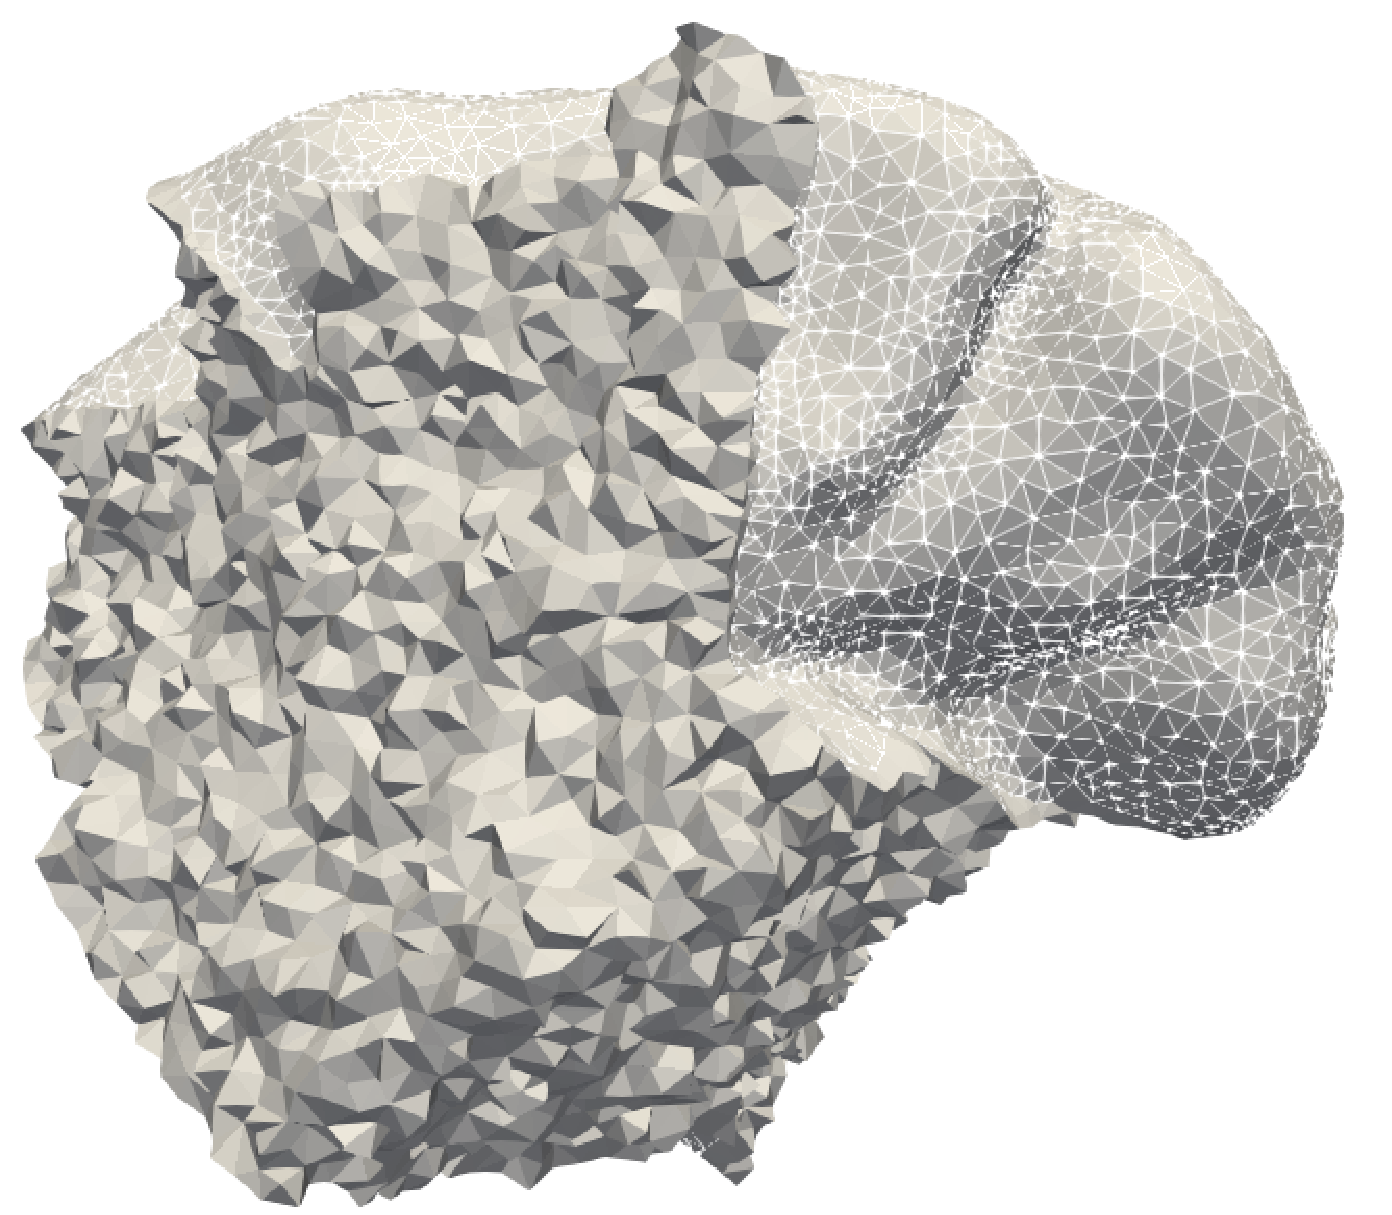
\includegraphics[width=0.4\textwidth]{brain_1_cropped.pdf} &
        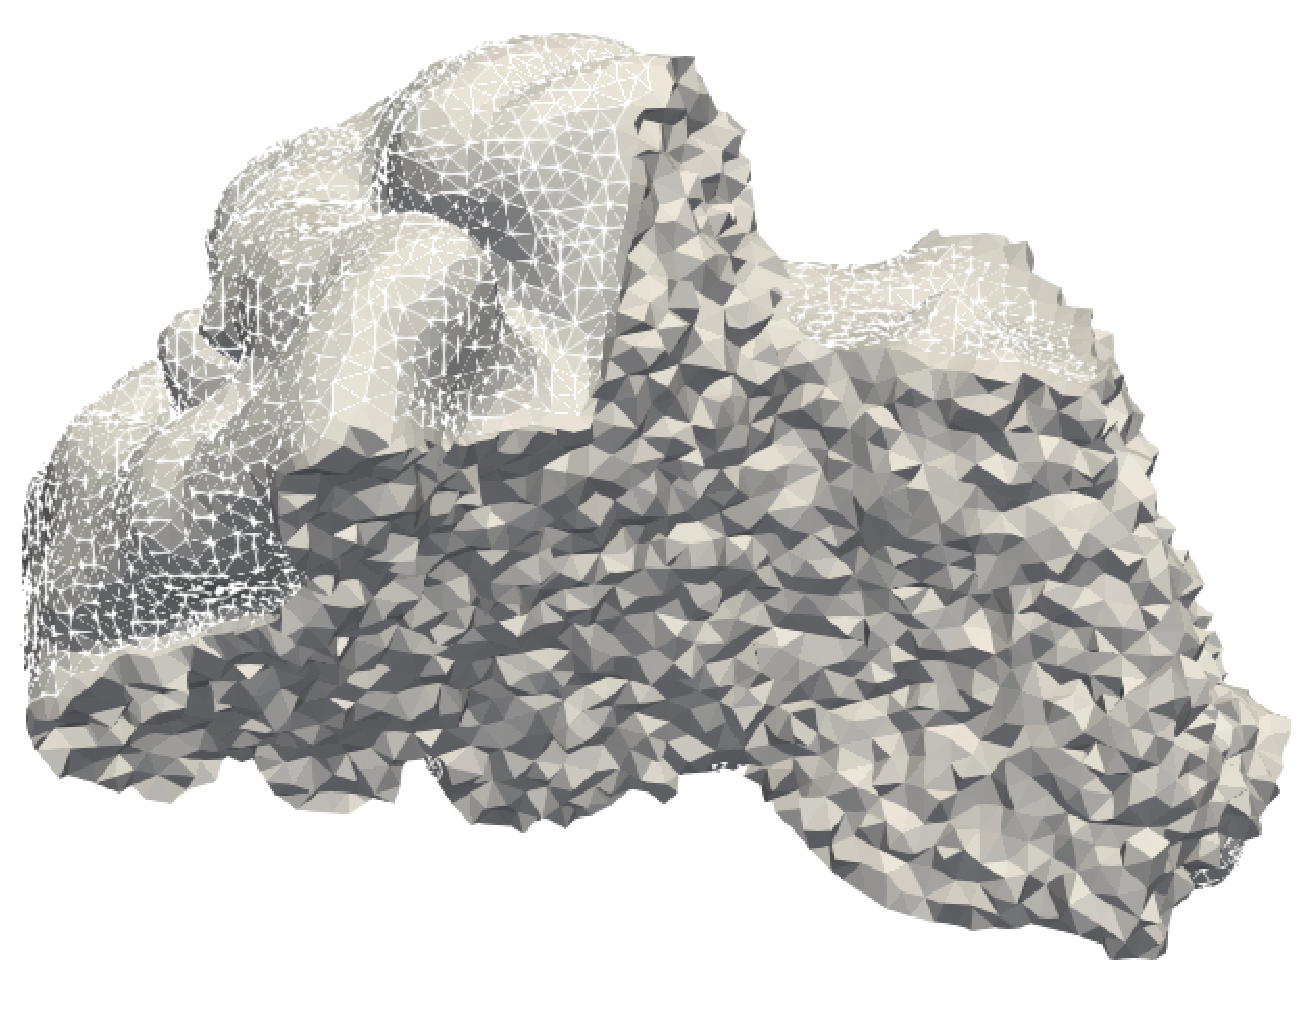
\includegraphics[width=0.4\textwidth]{brain_2_cropped.pdf}   \\
        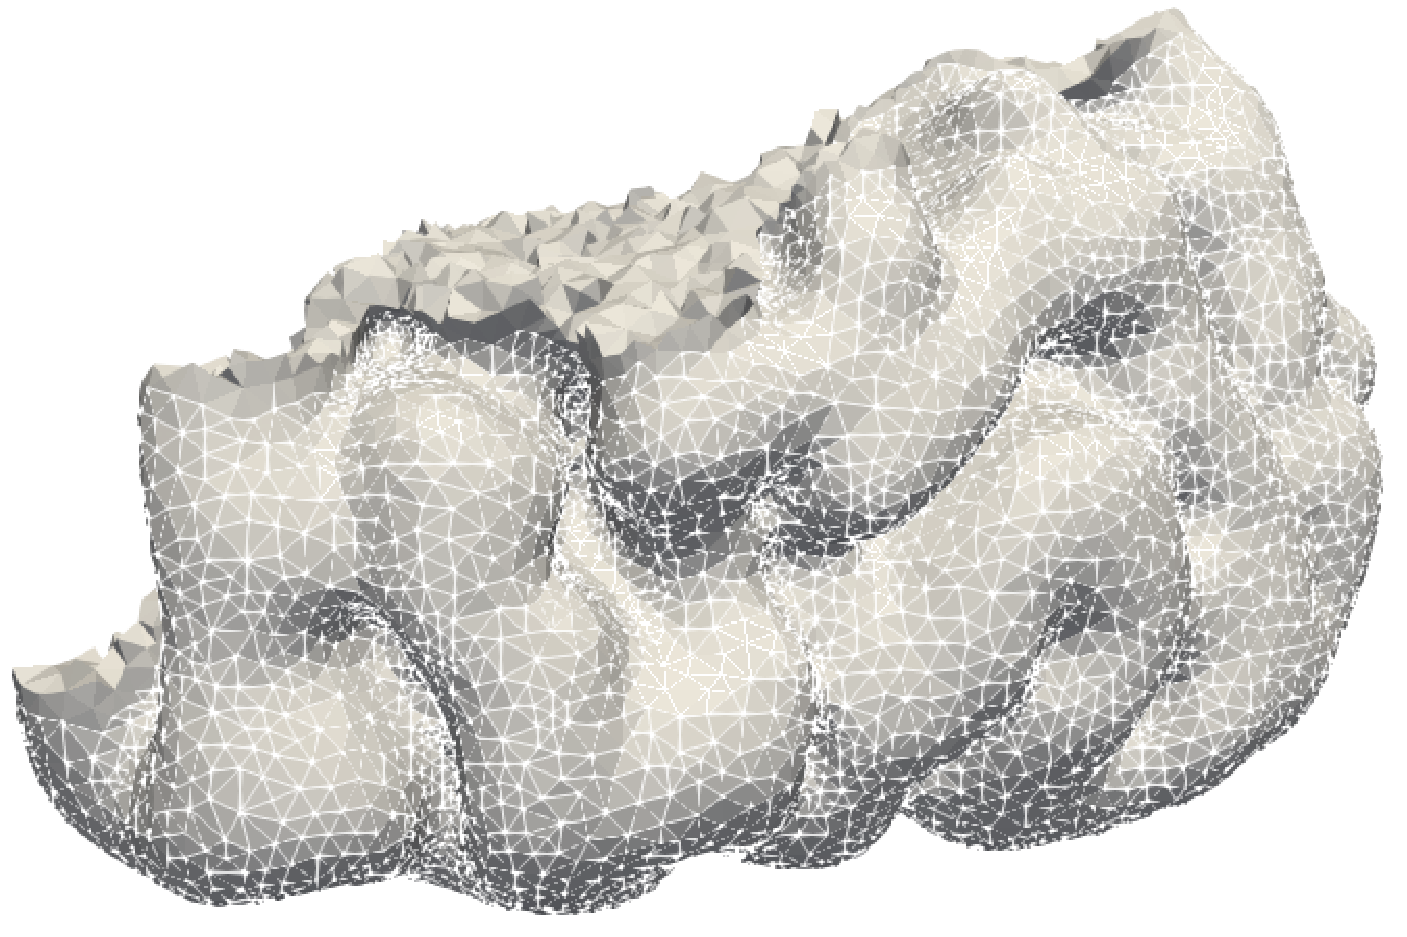
\includegraphics[width=0.4\textwidth]{brain_3_cropped.pdf} &
        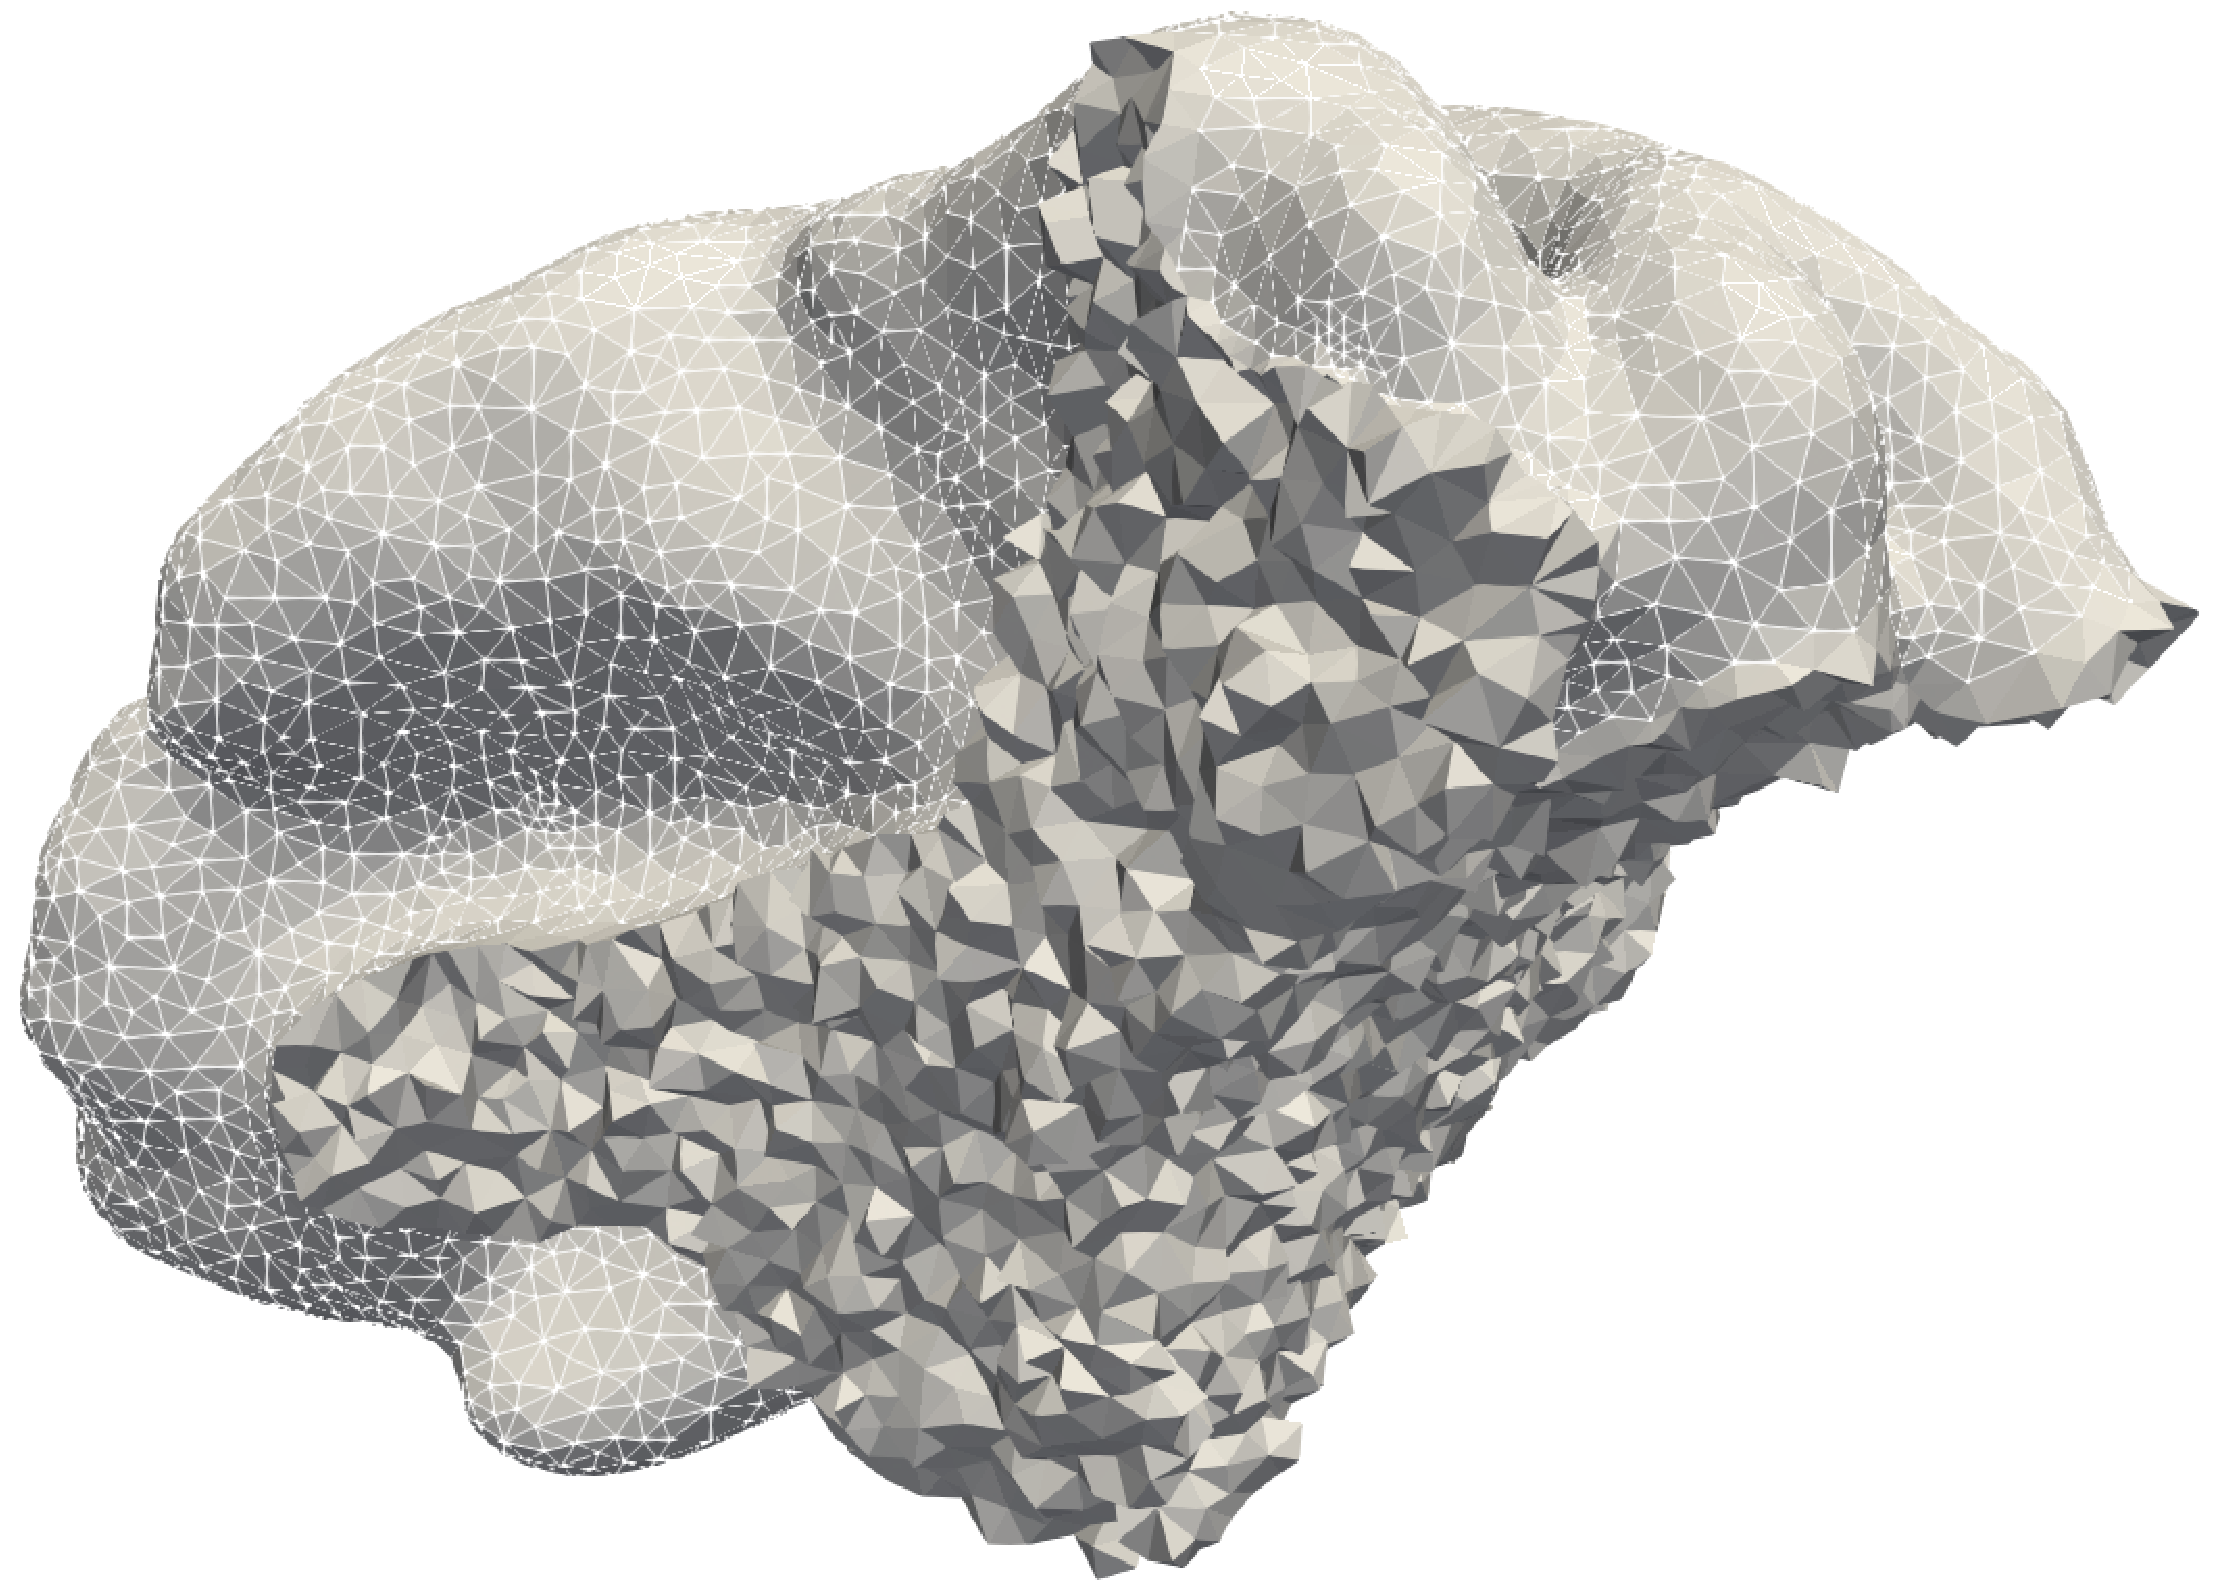
\includegraphics[width=0.4\textwidth]{brain_4_cropped.pdf}   \\
    \end{tabular}
    \caption{Visualizations of the partitions when N=4, for an initial brain mesh comprising $2\,375\,673$ tetrahedra.}
    \label{fig:partitioned_meshes}
\end{figure}

\noindent A possible workflow for this feature is summarized in the following code snippet:
\begin{lstlisting}[caption=Creating a \texttt{p::f::T} object from partitioned Gmsh files]
// Assume partitioned Gmsh files defined in MESH_DIR
static constexpr unsigned int dim = 3; // Dimension of the mesh
MPI_Comm mpi_comm = MPI_COMM_WORLD; // MPI communicator
parallel::fullydistributed::Triangulation<dim> tria(mpi_comm);
GridIn<dim>::read_partitioned_msh(tria,
                                  mpi_comm,
                                  MESH_DIR "/brain");
\end{lstlisting}


\noindent The integration of this new feature into deal.II is documented in
pull request \#18759 (\url{https://github.com/dealii/dealii/pull/18759}), and is
currently under review.

\begin{thebibliography}{10}
    \bibitem{gmsh} Geuzaine, C. and Remacle, J.-F., Gmsh: A 3-D finite element mesh generator with built-in pre- and post-processing facilities. Int. J. Numer. Meth. Engng., 79: 1309-1331, 2009.
\end{thebibliography}


\newpage

\section{{Conclusion}} \label{sec:conclusion}

\lipsum[20]

\label{MyLastPage}

\end{document}

%%% Local Variables:
%%% mode: LaTeX
%%% TeX-master: t
%%% End:
